\chapter{Metodologia}

\noindent Neste capítulo é descrita a aplicação das técnicas de Gerenciamento de Serviços de \acrshort{ti} \acrshort{itil} v3 e Engenharia de \textit{Software} retratadas no Capítulo 2 (Fundamentação Teórica). O objetivo deste capítulo é apresentar as metodologias adotadas na etapa de concepção do sistema ``\acrshort{uft} Serviços'', englobando o desenvolvimento das funcionalidades do sistema e os procedimentos adotados para a implantação do \textit{software}.

O capítulo está dividido em cinco seções, sendo elas: Desenvolvimento do Sistema, Ambiente Computacional, Métodos, Diagramas \gls{uml} e Ferramentas e Materiais. Na seção Desenvolvimento são expostos os conceitos utilizados para a criação e publicação do \textit{software} em produção, e apresentadas ferramentas de auxílio à implementação utilizadas no desenvolvimento do sistema. Por sua vez, na seção Ambiente Computacional, apresenta-se  a infraestrutura computacional de apoio exercida neste projeto. Já em Métodos, é demonstrada a utilização prática dos conceitos descritos na Fundamentação Teórica e a metodologia utilizada para aplicação do Teste de Usabilidade, o \textit{System Usability Scale}. Na seção referente à Diagramas  \acrshort{uml}, apresenta-se o Diagrama de Caso de Uso, Diagrama de Classe, Diagrama de Atividades e Diagrama de Implantação que foram utilizados como base para construção do sistema. Por último, em Ferramentas e Materiais, têm-se as principais ferramentas utilizadas no projeto, suas respectivas versões e as motivações para a escolha de cada uma delas.

\section{Desenvolvimento do Sistema}

\noindent Para o desenvolvimento do sistema ``\acrshort{uft} Serviços'' foram utilizados conceitos de desenvolvimento de software relativos à ferramentas de controle de versão de código fonte, testes unitários e automatização de deploy, apropriando-se do conceito de integração contínua de software. Deve-se salientar que estas abordagens estão integradas com a metodologia de desenvolvimento \textit{Scrum} utilizada para a construção deste trabalho.

A figura \ref{fluxograma-dev} demonstra o modelo adotado para o desenvolvimento do sistema, cujo modelo determina que a cada \textit{backlog} definido no \textit{sprint} sejam realizados todos os procedimentos presentes no fluxograma apresentado. 

O primeiro passo, após a definição da tarefa a ser realizada (\textit{backlog}), consiste na prototipação, incorporando as novas telas e funcionalidades do sistema. Após findada essa etapa,  é feita a codificação das novas funcionalidades do \textit{software} e realizado um conjunto de testes para verificar a ocorrência de alguma eventual falha. Em caso da ocorrência de algum problema no sistema, o desenvolvedor irá retornar para a etapa de codificação para que seja feita a correção da falha encontrada.

\begin{figure}[!h]
  \centering
  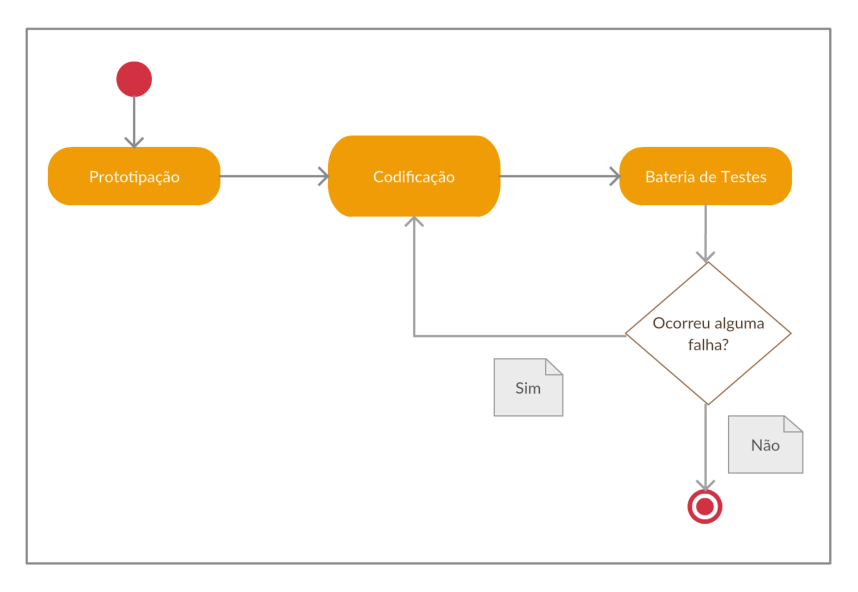
\includegraphics[width=.7\textwidth]{figuras/fluxograma_dev.eps} 
  \caption{Fluxograma de Desenvolvimento ``\acrshort{uft} Serviços''.}
  \label{fluxograma-dev} 
\end{figure} 

Conforme a Figura \ref{fluxograma-dev}, o modelo adotado para o desenvolvimento deste projeto propõe uma integração entre a metodologia de desenvolvimento ágil \textit{Scrum} e as boas práticas de desenvolvimento \textit{software}, utilizando-se de testes unitários e a criação de protótipos para validação de novas funcionalidades do sistema.

\section{Ambiente Computacional}

\noindent Nesta seção são demonstrados os ambientes computacionais utilizados para a construção (etapa de desenvolvimento) e funcionamento em produção do sistema ``\acrshort{uft} Serviços''. Desde a concepção deste projeto foi realizada uma pesquisa sobre quais tecnologias e conjunto de ferramentas de desenvolvimento de \textit{software} que possibilitaria a criação de um ambiente de programação flexível e que viabilizasse o gerenciamento de projetos de \textit{software} em equipe. Após a realização desta pesquisa foi escolhido o GIT\footnote{GIT: https://git-scm.com/} como ferramenta para o controle de versão do código fonte do projeto, tendo sua hospedagem feita em um conjunto de repositórios remotos de acesso privado no sistema Bitbucket\footnote{Bitbucket: https://bitbucket.org/}.

O motivo da escolha do GIT como sistema para o controle de versão se dá pelo fato dele ser uma das ferramentas mais consolidadas de versionamento de código fonte \cite{gitcontrole}. Sendo que, a motivação para a escolha do Bitbucket veio pela razão dele ser uma plataforma \textit{web} para hospedagem de projetos que utilizam o GIT, que tem como principal característica a criação ilimitada e gratuita de repositórios privados de código fonte \cite{bitbucket}.

Em conjunto com o GIT, foi adotado o conceito de integração contínua de desenvolvimento de \textit{software} através da ferramenta Jenkins\footnote{Jenkins: https://jenkins.io/}. O motivo para a escolha deste conceito se deu pelo fato da integração contínua ser uma prática que visa a integração frequente (várias vezes ao dia) de pequenas partes de código ao repositório principal de código-fonte, uma vez que, integrar pequenas partes facilita o tratamento dos possíveis problemas de integração, do que quando se integra partes maiores.

\subsection*{Ambiente de Desenvolvimento} 

\noindent O ambiente de desenvolvimento do ``\acrshort{uft} Serviços'' foi construído com base na arquitetura de desenvolvimento de aplicações corporativas \textit{Java Enterprise Edition} (Java EE)\footnote{Java EE: http://www.oracle.com/technetwork/java/javaee/overview/index.html}, padrão este que foi utilizado como suporte para a construção do sistema \textit{web} administrativo e aplicação de comunicação \acrshort{rest} API. 

Para o desenvolvimento do ambiente móvel foi utilizado o \gls{sdk}, disponibilizado pelo Google\footnote{Google: http://www.google.com} como padrão para construção de aplicações para o sistema operacional móvel Android\footnote{Android: https://www.android.com/}. Sendo que, uma característica presente em todas as aplicações descritas neste projeto está na utilização da linguagem de programação Java\footnote{Java: https://www.java.com}, como padrão de desenvolvimento de ambos os sistemas. 

A Figura \ref{ambiente_dev} demonstra o funcionamento do ambiente de desenvolvimento usado para a construção do sistema ``\acrshort{uft} Serviços''. O fluxo de programação inicia a partir do computador de desenvolvimento, onde estão instalados os ambientes de desenvolvimento integrado (IDE) Netbeans\footnote{Netbeans: https://netbeans.org/} e o Android Studio\footnote{Android Studio: https://developer.android.com/studio/index.html}, bem como o banco de dados necessário para que seja possível simular o ambiente de produção na máquina do programador. 

Na máquina do desenvolvedor está instalado o servidor \textit{web} \textit{Container} Java Jboss Wildfly\footnote{Wildfly: http://wildfly.org/}, servidor este que é responsável por receber todas as requisições \gls{http} do sistema \textit{web} administrativo, bem como todas as requisições feitas pelo aplicativo móvel Android presente nos \textit{smartphones} dos usuários. 

O GIT é utilizado para efetuar o controle de versão tanto do código fonte do aplicativo Android, como do sistema \textit{web}. Sendo que, todos esses repositórios estão também disponíveis remotamente no sistema Bitbucket, podendo estes serem acessados pelos programadores envolvidos no projeto que tenham suas respectivas permissões de acesso.

\begin{figure}[H]
  \centering
  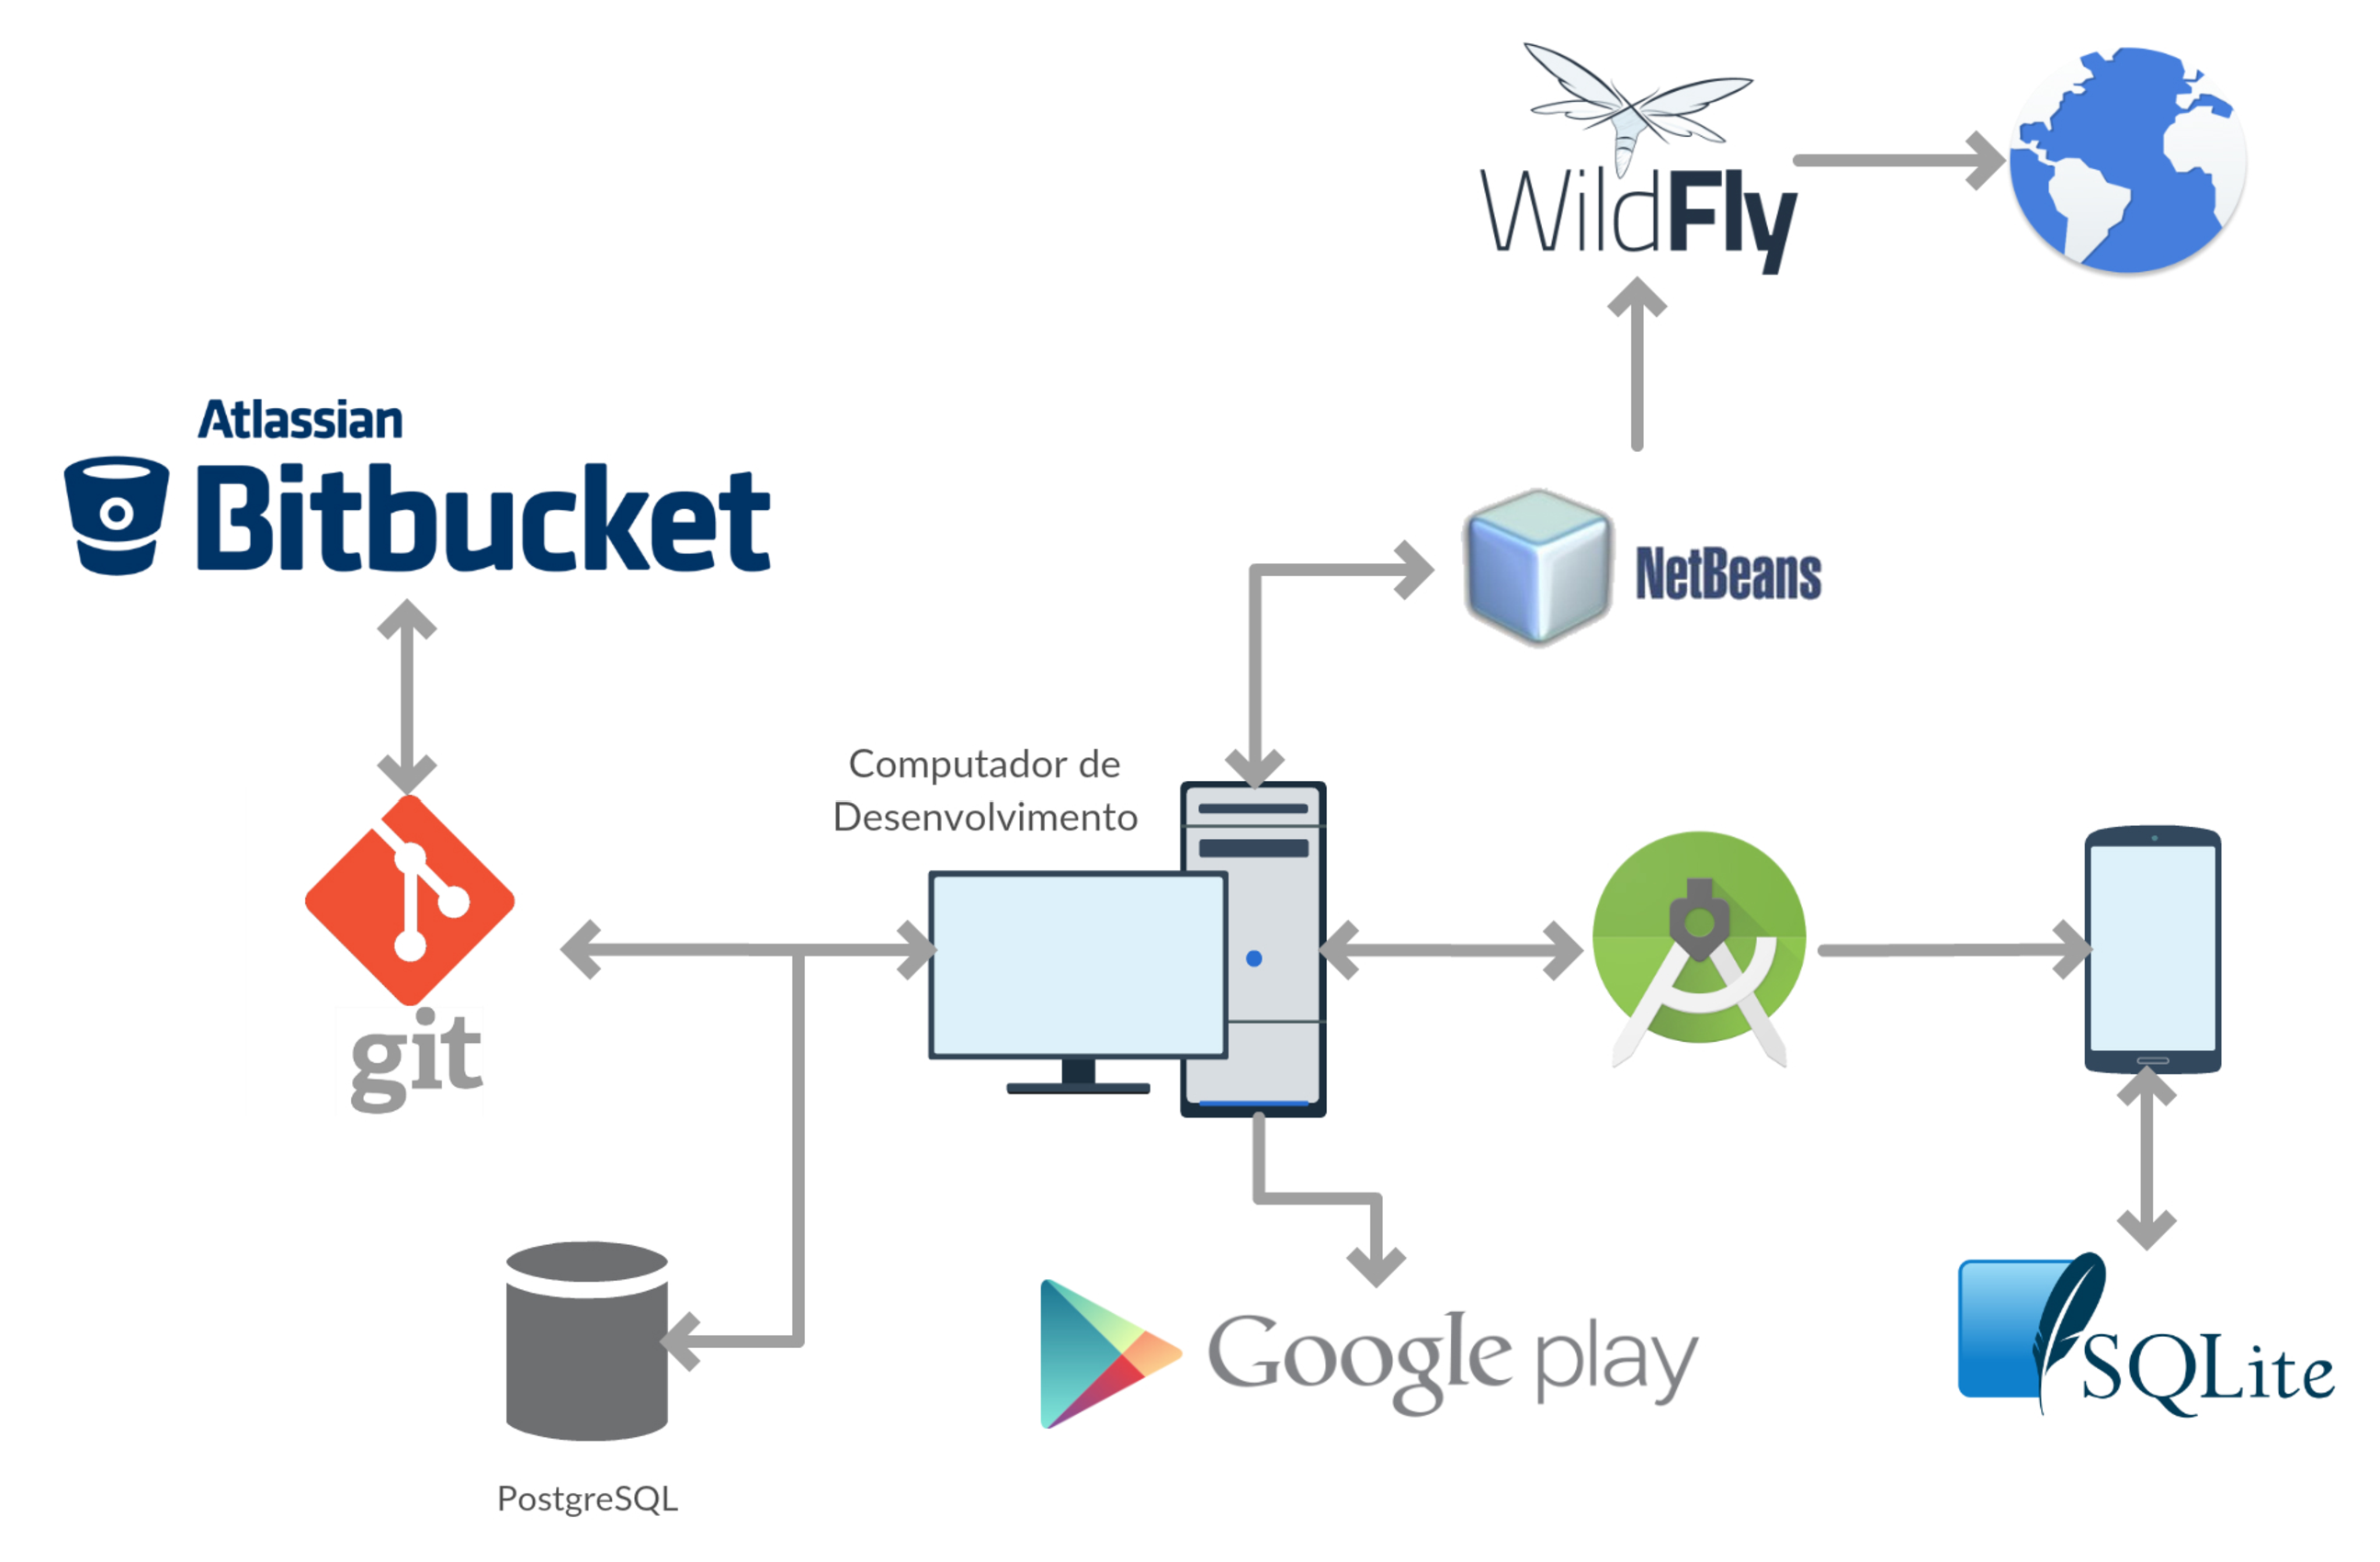
\includegraphics[width=0.7\textwidth]{figuras/develop.eps} 
  \caption{Ambiente de Desenvolvimento ``\acrshort{uft} Serviços''.}
  \label{ambiente_dev} 
\end{figure}

\subsection*{Ambiente de Produção}

\noindent O ambiente de produção foi montado de forma a automatizar as tarefas de atualização do Sistema \textit{web} administrativo do ``\acrshort{uft} Serviços''. O ambiente se concentra basicamente em três importantes servidores, sendo eles o Servidor de Banco de Dados, Servidor de Aplicação e Servidor de Integração Contínua.

A Figura \ref{ambiente_prod} demonstra o funcionamento do ambiente de produção, onde cada um dos servidores presentes desempenha um papel fundamental para o funcionamento do sistema. No servidor de banco de dados, onde está instalado o Banco de Dados Relacional PostgreSQL, há todas as informações dos chamados realizados pelo sistema móvel, e o histórico dos encaminhamentos realizados pelos usuários com acesso ao sistema \textit{web} administrativo. 

No Servidor de Aplicação (Wildfly), é onde fica hospedado a aplicação \textit{web} responsável por hospedar o sistema ``\acrshort{uft} Serviços'', além dele ser o responsável pela comunicação com o servidor de Banco de Dados do sistema e aplicativo móvel Android.

O Servidor de Integração Contínua é responsável por monitorar as modificações realizadas no repositório remoto no Bitbucket, onde a cada \textit{release}/\textit{commit} do \textit{software} ele é responsável por realizar o \textit{build} (etapa de compilação) e a execução de testes automatizados, através da definição de testes unitários definido pela a equipe de desenvolvedores. Sendo que, caso não ocorra nenhum erro durante este processo, é feito a atualização do sistema \textit{web} (deploy) no servidor de aplicação Wildfly.

\begin{figure}[H]
  \centering
  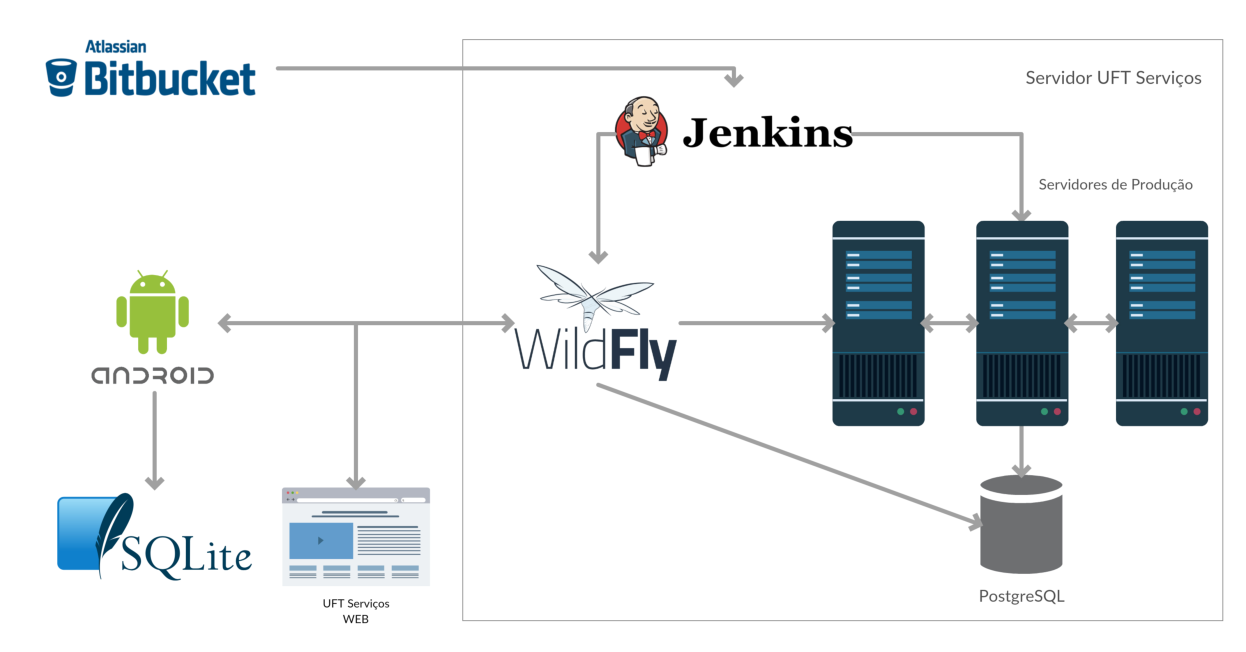
\includegraphics[width=0.7\textwidth]{figuras/production.eps} 
  \caption{Ambiente de Produção ``\acrshort{uft} Serviços''.}
  \label{ambiente_prod} 
\end{figure}

\section{Métodos}

\noindent Nesta seção é demonstrado os métodos aplicados para a construção e avaliação da etapa de desenvolvimento e implantação do sistema ``\acrshort{uft} Serviços''. Onde o objetivo deste capítulo é apresentar a aplicação dos métodos que foram retratados no Capítulo de Fundamentação Teórica, como a utilização do \acrshort{itil} v3, o modelo de desenvolvimento ágil \textit{Scrum} e a técnica utilizada para a avaliação da usabilidade do sistema, o \textit{System Usability Scale}.

\subsection*{Ciclo de Vida de Serviços (\acrshort{itil} v3)}

\noindent Dado as etapas do ciclo de vida de serviços do \acrshort{itil} v3 descrito na Fundamentação Teórica, foi realizada uma análise sobre quais de suas principais práticas seriam aplicadas neste projeto. A utilização das práticas do \acrshort{itil} v3 adotadas neste trabalho foi feita através da escolha de suas principais técnicas, sendo levado em consideração também o tempo para execução destas técnicas e que elas estejam dentro de um tempo hábil de implantação do sistema. 

A Figura \ref{itil_aply} demonstra todos os processos presentes na fundamentação do \acrshort{itil} v3, onde cada um dos processos apresentados compõem o ciclo de vida de serviços apresentado no Capítulo 2.

\begin{figure}[H]
  \centering
  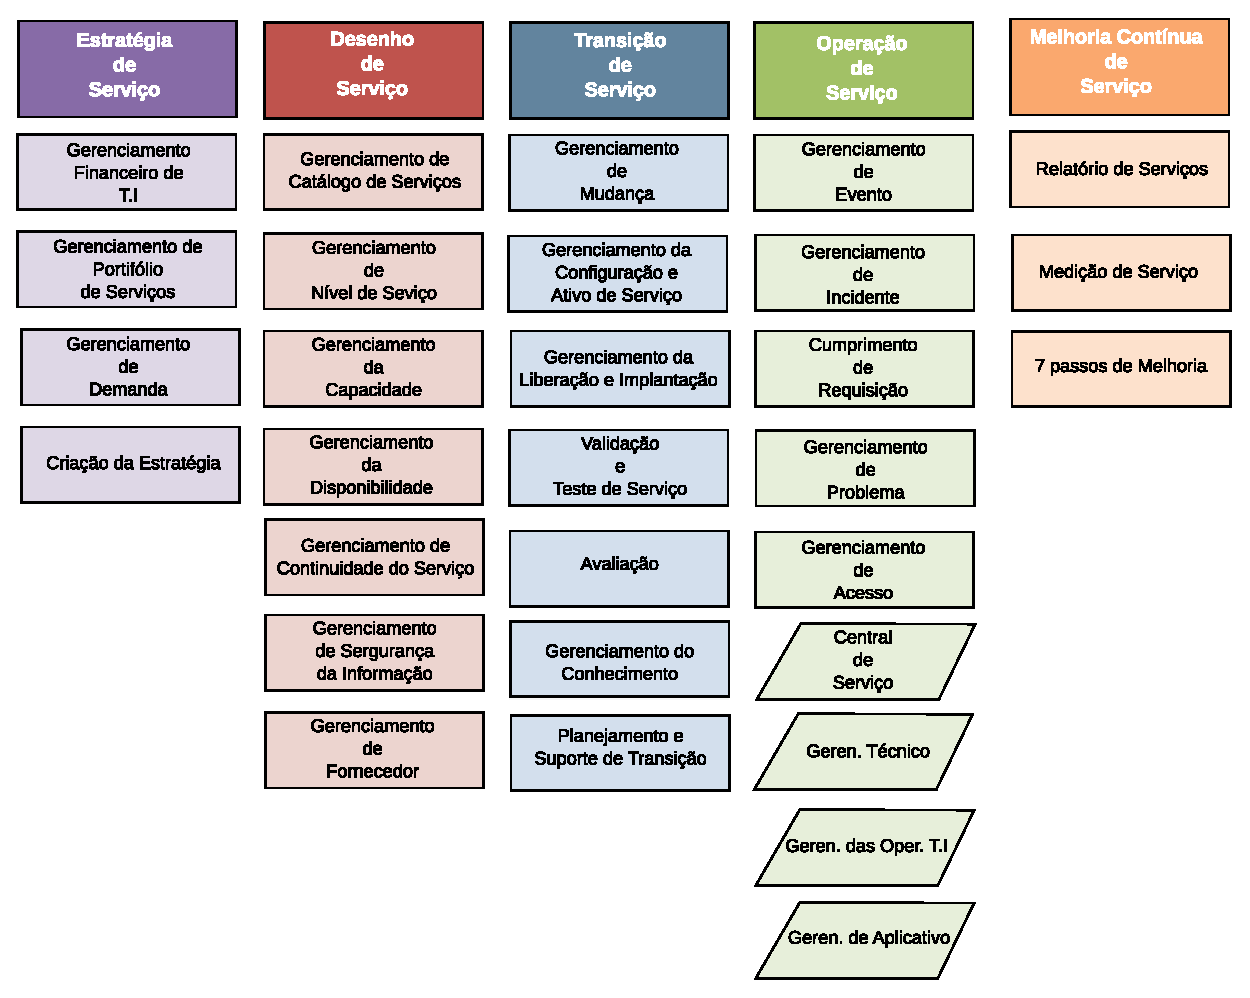
\includegraphics[width=0.7\textwidth]{figuras/itil_aply.eps} 
  \caption{Itens do Ciclo de Vida de Serviços \acrshort{itil} v3 (Adaptada de \cite{introductoryoverviewofitil}).}
  \label{itil_aply} 
\end{figure}

Após feita a análise sobre quais itens do \acrshort{itil} v3 seriam aplicados neste trabalho, foi decidido pela utilização das seguintes técnicas:

\begin{itemize}
    \item Estratégia de Serviços: através da Criação da Estratégia e Gerenciamento de Demanda;
    \item Desenho de Serviço: através do Gerenciamento de Nível de Serviço, Gerenciamento da Capacidade, Gerenciamento da Disponibilidade, Gerenciamento de Segurança da Informação e Gerenciamento de Fornecedor;
    \item Transição de Serviço: através do Gerenciamento de Mudança, Validação e Teste de Serviço, Avaliação e Gerenciamento do Conhecimento; e
    \item Melhoria Contínua de Serviço: através da Medição de Serviço.
\end{itemize}

\subsection*{Estratégia de Serviço}

\noindent Na etapa de Estratégia de Serviço foi utilizada o conceito de Gerenciamento de Demanda e Criação de Estratégia, que serviu como base para a criação da Estratégia de Serviço do sistema ``\acrshort{uft} Serviços''.

Em Gerenciamento de Demanda foi definido através da criação do Acordo de Nível de Serviço, onde foi definido como será realizado o gerenciamento da demanda do serviços presentes no acordo após a implantação do sistema ``\acrshort{uft} Serviços''.

Foi através da etapa de Criação de Estratégia que foi possível criar as perspectivas estratégicas de utilização do sistema ``\acrshort{uft} Serviços''. Sendo que a criação da estratégia de implantação deste projeto se baseou no modelo dos 4 Ps da estratégia, que é caracterizado por \cite{servicestrategy}:

\begin{itemize}
    \item Perspectiva: Onde é definido os valores da organização, através da definição da missão, visão e valores;
    \item Posição: Caracterizado pelo posicionamento da organização frente aos problemas enfrentados;
    \item Plano: Através da aplicação de um conjunto de estratégias para alcançar a visão e os objetivos da organização; e
    \item Padrão: Tem como característica a aplicação de processos e organizações para que os objetivos sejam satisfeitos.
\end{itemize}

\subsection*{Desenho de Serviço}

\noindent Durante a etapa de Desenho de Serviço, foi empregado os conceitos de Gerenciamento de Nível de Serviço, Gerenciamento de Capacidade, Gerenciamento de Disponibilidade, Gerenciamento de Segurança da Informação e Gerenciamento de Fornecedor. Cada um dos gerenciamentos mencionados foram aplicados durante a etapa de planejamento de desenvolvimento do sistema ``\acrshort{uft} Serviços''.

No Gerenciamento de Nível de Serviço, foi firmado um acordo entre os clientes do sistema e fornecedores, a partir da criação do \acrshort{ti} disponível no Apêndice IV. A partir da criação deste documento foram definidas informações como as responsabilidades que os prestadores de serviço de \acrshort{ti} tem com seus clientes e fornecedores, através da definição das responsabilidades em que todos os evolvidos tem com este acordo.

Na etapa de Gerenciamento de Capacidade, foram definidas informações que visam garantir que os serviços de \acrshort{ti} e infraestrutura tenham capacidade de atender os requisitos com relação a capacidade e que as informações presentes no gerenciamento de capacidade estejam de acordo com as necessidades dos utilizadores do sistema.

Como parte do Gerenciamento de Disponibilidade do sistema, foi criado em forma de documento o Plano de Gestão de Disponibilidade do sistema ``\acrshort{uft} Serviços'' neste documento estão presentes informações que contém um conjunto de direcionamentos que visam manter o alinhamento das estratégias de negócio da organização que foram definidas na \acrshort{ti}.

Na fase de Gerenciamento de Segurança da Informação, foram definidas as medidas de segurança de forma que haja um alinhamento com as necessidades da organização e com os requisitos de privacidade dos dados armazenados dos usuários. Por conta de se tratar de modelo incremental de segurança, foram definidos inicialmente os requisitos de autenticação do sistema e que os dados referentes a abertura de um chamado sejam apenas compartilhados, entre o solicitante e o administrador do sistema.

A etapa de Gerenciamento de Fornecedor foi utilizada para garantir que os fornecedores externos ao serviço oferecido pelo sistema estejam de acordo com as metas e expectativas de negócio da organização e de seus clientes. Foi através da definição do gerenciamento de fornecedores que foi possível gerenciar o desempenho dos fornecedores e negociação de contratos durante o ciclo de vida do acordo.

\subsection*{Transição de Serviço}

\noindent Na etapa de Transição de Serviço foi utilizado os conceitos de Gerenciamento de Mudanças, Validação e Teste de Serviço, Avaliação e Gerenciamento do Comportamento. Sendo que cada uma das etapas foram aplicadas durante a fase de transição de serviço do sistema.

A fase de Gerenciamento de Mudanças foi aplicada para minimizar o impacto causado pela necessidade da aplicação de mudanças críticas no sistema e seu principal objetivo é otimizar a exposição a riscos e prevenir o surgimento de transtornos aos utilizadores do \textit{software}.

A utilização de Validação e Testes de Serviço foi de grande importância para o planejamento da aplicação de novas funcionalidades e correções dos erros encontrados no sistema. Foi através desta etapa em conjunto com práticas de programação orientada a testes e integração contínua do \textit{software}, que foi possível fazer uma validação mais segura referente a atualização do sistema em produção de forma automatizada.

Na fase de Avaliação, utilizou-se os \textit{feedbacks} das  a apresentação das novas funcionalidades do sistema aos envolvidos no projeto e as sugestões de mudanças propostas pelos clientes do sistema. A etapa de avaliação foi de grande importância, pois ela forneceu um conjunto de informações com relação à experiência do usuário que influenciaram na criação de adaptações das funcionalidades do sistema.

A etapa de Gerenciamento do Conhecimento foi aplicada para a melhoria da gestão de tomada de decisão, assegurando que informações precisas estejam disponível de forma clara em todo o ciclo de vida de serviços. A utilização da gestão de conhecimento foi de grande importância durante a implantação do sistema ``\acrshort{uft} Serviços'', pois a partir da gestão efetiva do conhecimento foi possível criar uma documentação clara contendo as informações referentes ao desenvolvimento e implantação do sistema.

\subsection*{Melhoria Contínua de Serviço}

\noindent A etapa de Melhoria Contínua do Serviço foi uma das etapas mais importantes da aplicação das práticas do \acrshort{itil} v3 neste projeto, foi a partir dela que foi possível mensurar os serviços oferecidos pelo sistema através da etapa de Medição do Serviço.

Na etapa de Medição do Serviço, foi possível mensurar através de ferramentas de monitoramento, o comportamento do sistema e de seus usuários, através do monitoramento da infraestrutura de \textit{hardware} que mantém o sistema no ar e das informações básicas sobre o usuário, como a idade, o sexo e o histórico de navegação durante a utilização do aplicativo móvel.

Uma outra forma de medição do serviço oferecido pelo sistema foi a partir da aplicação do teste de usabilidade  \acrshort{sus}, sua aplicação em conjunto com as outras informações geradas pela medição do serviço foi de grande importância, pois possibilitou uma avaliação efetiva sobre os ganhos obtido pela implantação do sistema.

\subsection*{Desenvolvimento Ágil (\textit{Scrum})}

\noindent A utilização \textit{Scrum} foi crucial para a organização das atividades necessárias para a conclusão do desenvolvimento do sistema, em conjunto com as práticas de desenvolvimento ágil \textit{Scrum} foi utilizado o modelo de organização de tarefas chamado \textit{Kanban} \cite{anderson2010kanban}. A Figura \ref{quadro-kanban} demonstra como é o funcionamento dessa técnica, onde basicamente as tarefas são divididas em três ou mais colunas contendo uma identificação única para um dado conjunto de tarefas, representada através de anotações em \textit{post-it}.

Neste projeto foi utilizado três colunas para representar as atividades realizadas, sendo elas tarefas: Á fazer, Em desenvolvimento e Finalizado. Na coluna de tarefas Á fazer é onde é colocada todas as novas tarefas a serem realizadas. Nas tarefas Em desenvolvimento é colocada todas as tarefas que foram iniciadas, mas ainda não foram concluídas. Na coluna Finalizado é colocada todas as tarefas que foram finalizadas. Para um melhor acompanhamento das demandas do sistema ``\acrshort{uft} Serviços'', foi utilizado a ferramenta colaborativa de organização de tarefas chamada Trello\footnote{Trello: https://trello.com/}.

\begin{figure}[H]
 \centering
 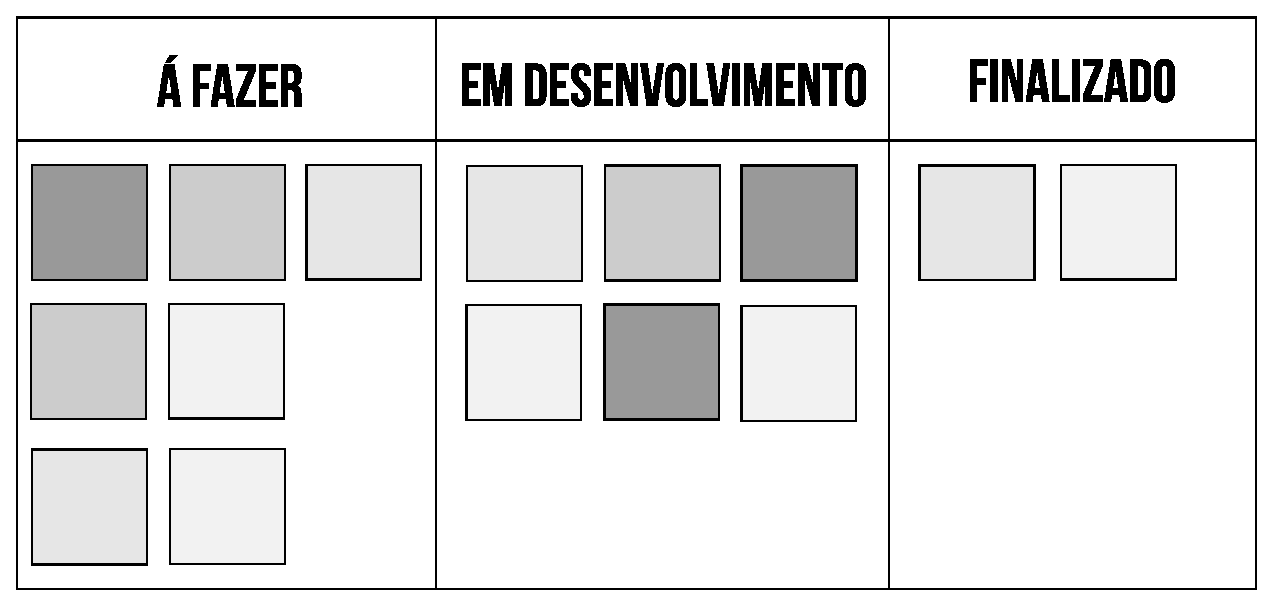
\includegraphics[width=0.7\textwidth]{figuras/kanban.eps} 
 \caption{Quadro de atividades Kanban.}
 \label{quadro-kanban} 
\end{figure}

Todas as atividades realizadas neste projeto foram baseadas na metodologia de desenvolvimento ágil \textit{Scrum}, através do conceito de organizações dos \textit{backlog} e das demandas a serem entregas a partir da definição dos \textit{sprints}, sendo que o acompanhamento do projeto foi feito a partir de reuniões periódicas em conjunto com os demais envolvidos no projeto.

\subsection*{Teste de Usabilidade (\textit{System Usability Scale})}

\noindent A realização do teste de usabilidade é um dos pontos fundamentais para avaliação do resultado do \textit{software} desenvolvido neste trabalho. Através da realização deste teste é possível identificar os principais pontos positivos e negativos com relação a usabilidade do sistema ``\acrshort{uft} Serviços'', podendo ser averiguado itens como a facilidade do uso do sistema, a eficiência e se o usuário se sente confortável em estar utilizando o sistema pela primeira vez.

O teste utilizado neste projeto é o \textit{System Usability Scale} (SUS) que consiste em um questionamento contendo 10 afirmativas que abrangem as seguintes possibilidade de respostas: Discordo Totalmente, Discordo, Neutro, Concordo e Concordo Totalmente. Uma característica importante do  \acrshort{sus} é que nele somente é permitido aos usuários uma única resposta por pergunta e que sua aplicação sempre ocorre logo após a utilização do sistema pelo usuário. O \acrshort{sus} se caracteriza como um modelo para averiguação da usabilidade que procura mensurar o nível de facilidade de uso de um sistema, tendo como foco em três pontos fundamentais que é a efetividade, eficiência e a satisfações dos usuários do sistema \cite{bangor2009determining}. No Apêndice II é apresentado o formulário utilizado para realização do teste de usabilidade.

Cada resposta feita no questionário do \acrshort{sus} tem uma escala de variação que vai de 1 a 5, onde 1 significa que o usuário discorda totalmente e 5 que ele concorda plenamente com o que está sendo questionado \cite{bangor2009determining}. 

Para saber se um sistema é de boa usabilidade ou não o \acrshort{sus} aplica o seguinte conjunto de regras: primeiramente é subtraído por 1 todas as respostas de questões de numeração ímpar (1, 3, 5, 7, 9) e subtraído por 5 todas as questões pares (2, 4, 6, 8, 10). Após fazer a devida subtração de cada item deve-se fazer um somatório dos valores obtidos de cada questão e multiplicar por 2.5, assim obtendo uma pontuação resultante variando do intervalo de 0 a 100. Para que um sistema seja caracterizado minimamente usável deve-se obter a pontuação mínima de 68 pontos, sendo que notas menores a 68 caracteriza o sistema avaliado como de baixa usabilidade \cite{Brooke:2013:SR:2817912.2817913}.

A Figura \ref{escala-sus} mostra a distribuição dos níveis de usabilidade do  \acrshort{sus}, como pode ser observado o  \acrshort{sus} possui uma escala que compreende os níveis F, D, C, B e A. Cada um dos níveis apresentados representa um intervalo de nota referente a nota obtida pela avaliação do  \acrshort{sus}, sendo a pior nota representada pela letra F e a melhor pela letra A.

\begin{figure}[H]
 \centering
 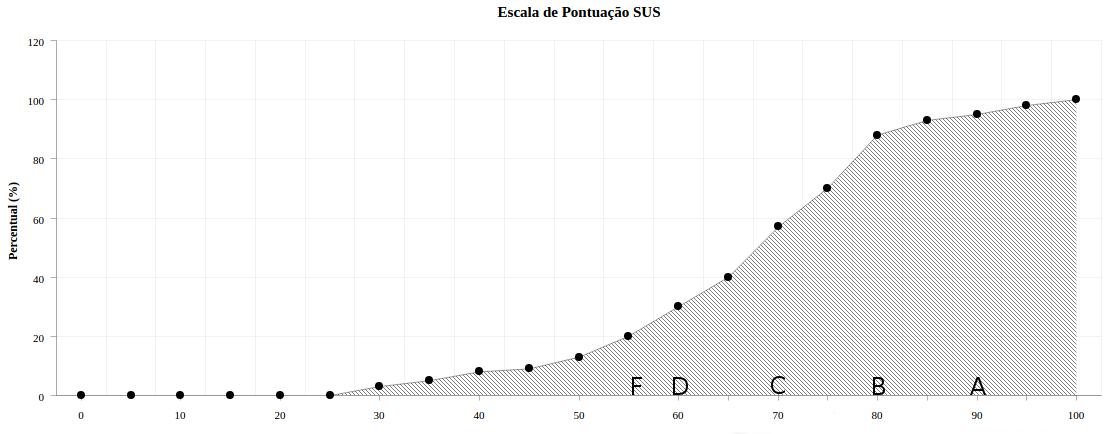
\includegraphics[width=1\textwidth]{figuras/escala_sus.png} 
 \caption{Distribuição dos níveis de usabilidade do \textit{System Usability Scale} (SUS) (Adaptado de \cite{bangor2009determining}).}
 \label{escala-sus} 
\end{figure}

Na Tabela \ref{tabela-sus} mostra a distribuição dos intervalos de notas do  \acrshort{sus} e suas respectivas classificações. Como pode ser observado, a classificação do  \acrshort{sus} pode variar entre cinco principais resultados, sendo eles: Ruim, Razoável, Bom, Excelente e Muito Excelente.

\begin{table}[H]
    \centering
    \small
    \begin{tabular}{|c|c|c|}
    \hline
    \multicolumn{1}{|l|}{Atribuição} & \multicolumn{1}{l|}{Classificação} & \multicolumn{1}{l|}{Variação de Nota} \\ \hline
    F                                & Ruim                               & x $\leq $ 60                        \\ \hline
    D                                & Razoável                           & 60  \textless x $\leq$ 70          \\ \hline
    C                                & Bom                                & 60 \textless x $\leq$ 80           \\ \hline
    B                                & Excelente                          & 80 \textless x $\leq$ 90           \\ \hline
    A                                & Muito Excelente                    & x $\geq$ 90                     \\ \hline
    \end{tabular}
    \caption{Tabela de classificação do \textit{System Usability Scale} (SUS).}
    \label{tabela-sus}
\end{table}

Como pode ser observado, o \acrshort{sus} classifica o sistema através da nota média obtida pela aplicação da fórmula descrita anteriormente no início desta seção. Sendo que, para valores menores que 60 o sistema é classificado como um \textit{software} de baixa usabilidade, se a nota for entre 60 e 70 ele é classificado como de usabilidade razoável, nota entre 60 e 80 o sistema é classificado como de boa usabilidade, se o resultado for entre 80 e 90 o sistema é classificado como de excelente usabilidade e por fim se a nota for maior que 90 o sistema é classificado como Muito Excelente no quesito usabilidade.

\section{Diagramas \acrshort{uml}}

\noindent Nesta seção são apresentados os diagramas \textit{Unified Modeling Language} (UML) utilizadas para criação do sistema ``\acrshort{uft} Serviços'', onde foi decidido devido a necessidade de que ocorra o desenvolvimento do sistema que esteja de acordo com o que foi planejado inicialmente no levantamento de requisito pela criação do Diagrama de Caso de Uso da utilização do sistema, o Diagrama de Classe (Sistema \textit{web} e \textit{Mobile}), o Diagrama de Atividade contendo as principais atividades da utilização do sistema e o Diagrama de Implantação.

\subsection*{Diagrama de Caso de Uso}

Para exemplificar melhor o \textit{workflow} de funcionamento do sistema ``\acrshort{uft} Serviços'' foi criado um diagrama geral de caso de uso, conforme apresentado na Figura \ref{diagram-uml-casodeuso}. Neste diagrama é demonstrado uma visão geral sobre os principais atores presentes na utilização do sistema, sendo eles o corpo docente, discente, técnico administrativo e a central de atendimento dos chamados.

\begin{figure}[H]
 \centering
 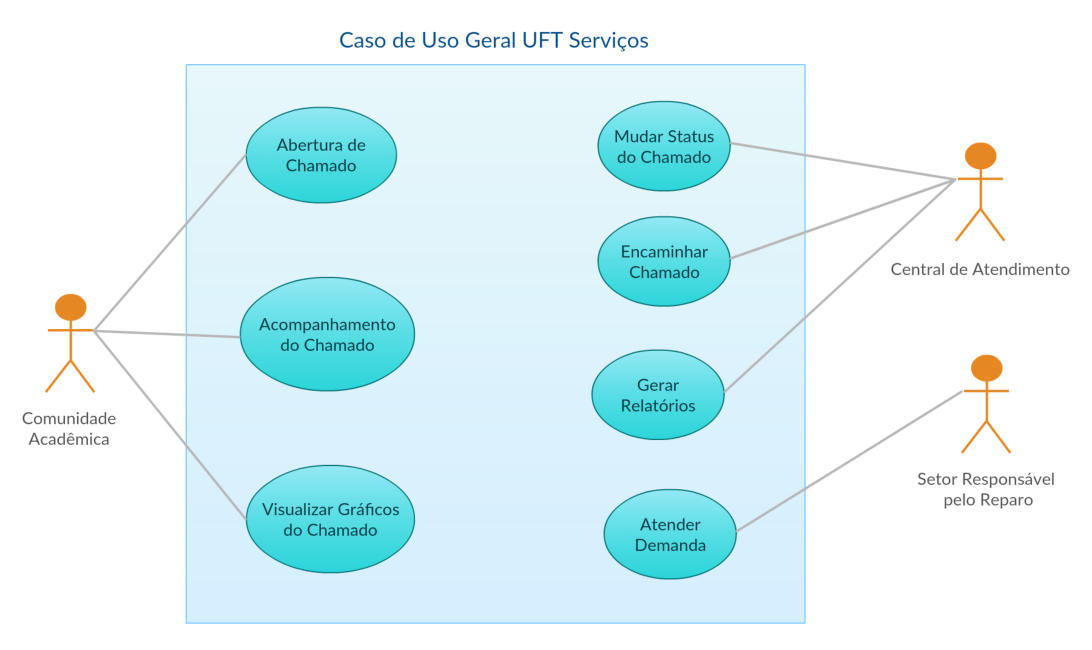
\includegraphics[width=1\textwidth]{figuras/uml-casodeuso.eps} 
 \caption{Diagrama de Caso de Uso Geral sistema ``\acrshort{uft} Serviços''.}
 \label{diagram-uml-casodeuso} 
\end{figure}

O diagrama demonstra todas as atividades que podem ser exercidas por cada um dos atores mencionados, como pode ser observado a comunidade acadêmica pode utilizar o sistema realizando chamados, acompanhando e fiscalizando a solução dos problemas além de poder visualizar os gráficos do chamado. Já na parte administrativa do sistema fica a cargo da Central de Atendimento realizar a mudança do estágio do chamado o seu encaminhamento e a geração dos relatórios, e por fim o ator intitulado Responsável pelo Reparo é responsável por estar executando a ordem de serviço.

\subsection*{Diagrama de Classe}

\noindent Nesta seção é apresentados os diagramas de classe do Sistema \textit{web} e do Sistema \textit{Mobile}, onde a partir da definição destes diagramas foram criadas as classes e a lógica de negócio da aplicação. Durante o desenvolvimento desta modelagem foi feito da forma mais enxuta possível, de forma que ao criar as classes do sistema não houvesse nenhuma dificuldade durante sua implementação, fornecendo um baixo acoplamento de código.

Como pode ser observado a seguir é mostrado os diagramas de classe que foram criados onde são demonstradas todas as principais classes de domínio que compõem o sistema ``\acrshort{uft} Serviços'', apresentando informações como os atributos e métodos pertencentes a cada uma das classes existentes em ambos os sistemas. A seguir as Figuras \ref{diagram-android} e \ref{diagram-web} é demonstrado os diagramas de classe do sistema.

O primeiro diagrama de atividade apresentado pela Figura \ref{diagram-android} é exemplificado o processo de abertura de um chamado pelos usuários do sistema através do aplicativo Android. O processo consiste na seleção de uma categoria de chamado cadastrado no sistema e a validação do formulário a partir do preenchimento de informações como o título, descrição, localização e foto do chamado. Após a validação do formulário de abertura do chamado as informações são então serializadas e enviadas pela rede para o servidor de aplicação do ``\acrshort{uft} Serviços''.

O diagrama apresentado na Figura \ref{diagram-web} apresenta o processo de cadastro e autenticação do usuário no aplicativo móvel, o processo consiste no preenchimento e validação do formulário de cadastro de usuário. Após a validação é enviado as informações para o servidor de aplicação é criado um usuário com o \textit{status} inativo e enviado um \textit{e-mail} de ativação do usuário, logo em seguida caso o usuário clique no \textit{link} de ativação o seu \textit{status} será mudado para ativo e com isso o usuário poderá logar no sistema a partir do aplicativo Android.

\begin{figure}[H]
 \centering
 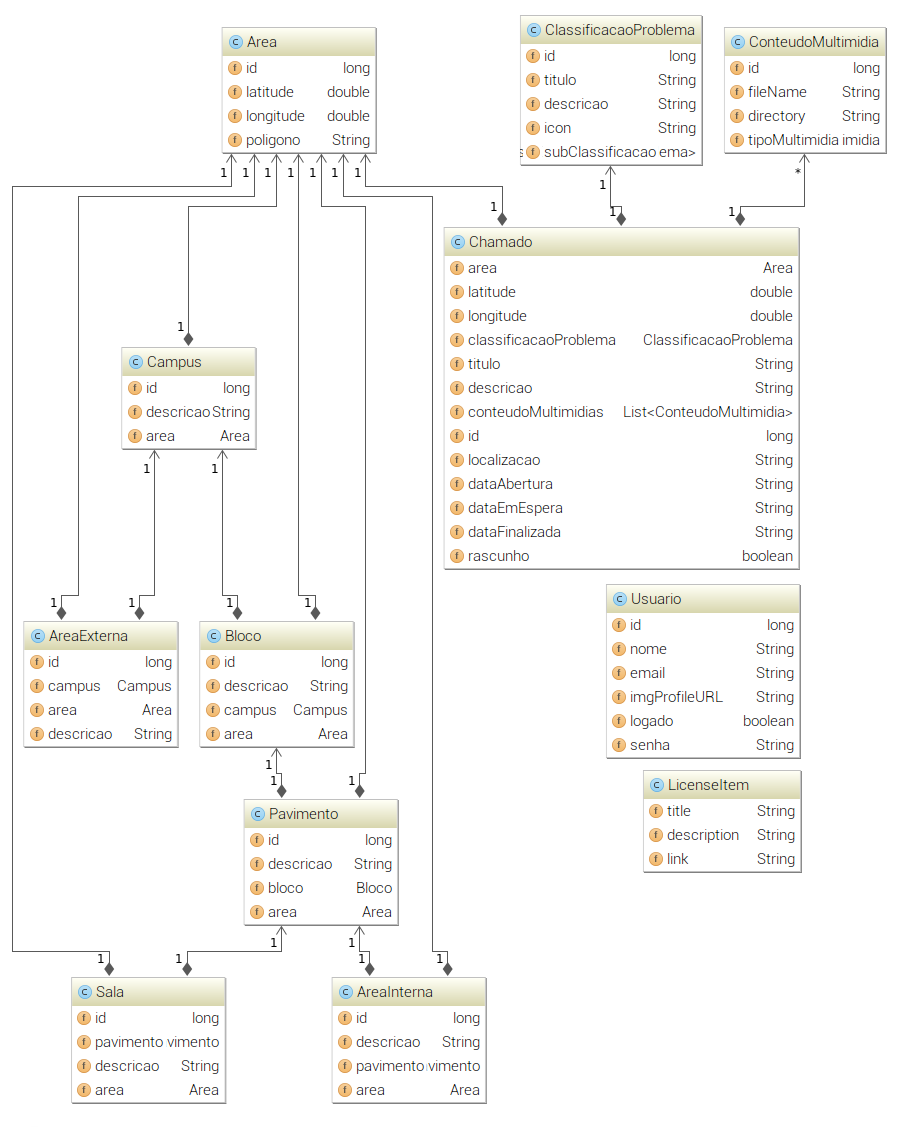
\includegraphics[angle=270, width=1\textwidth]{figuras/uft-servicos-android-diagram} 
 \caption{Diagrama de classes do sistema ``\acrshort{uft} Serviços'' Android.}
 \label{diagram-android} 
\end{figure}

\begin{figure}[H]
 \centering
 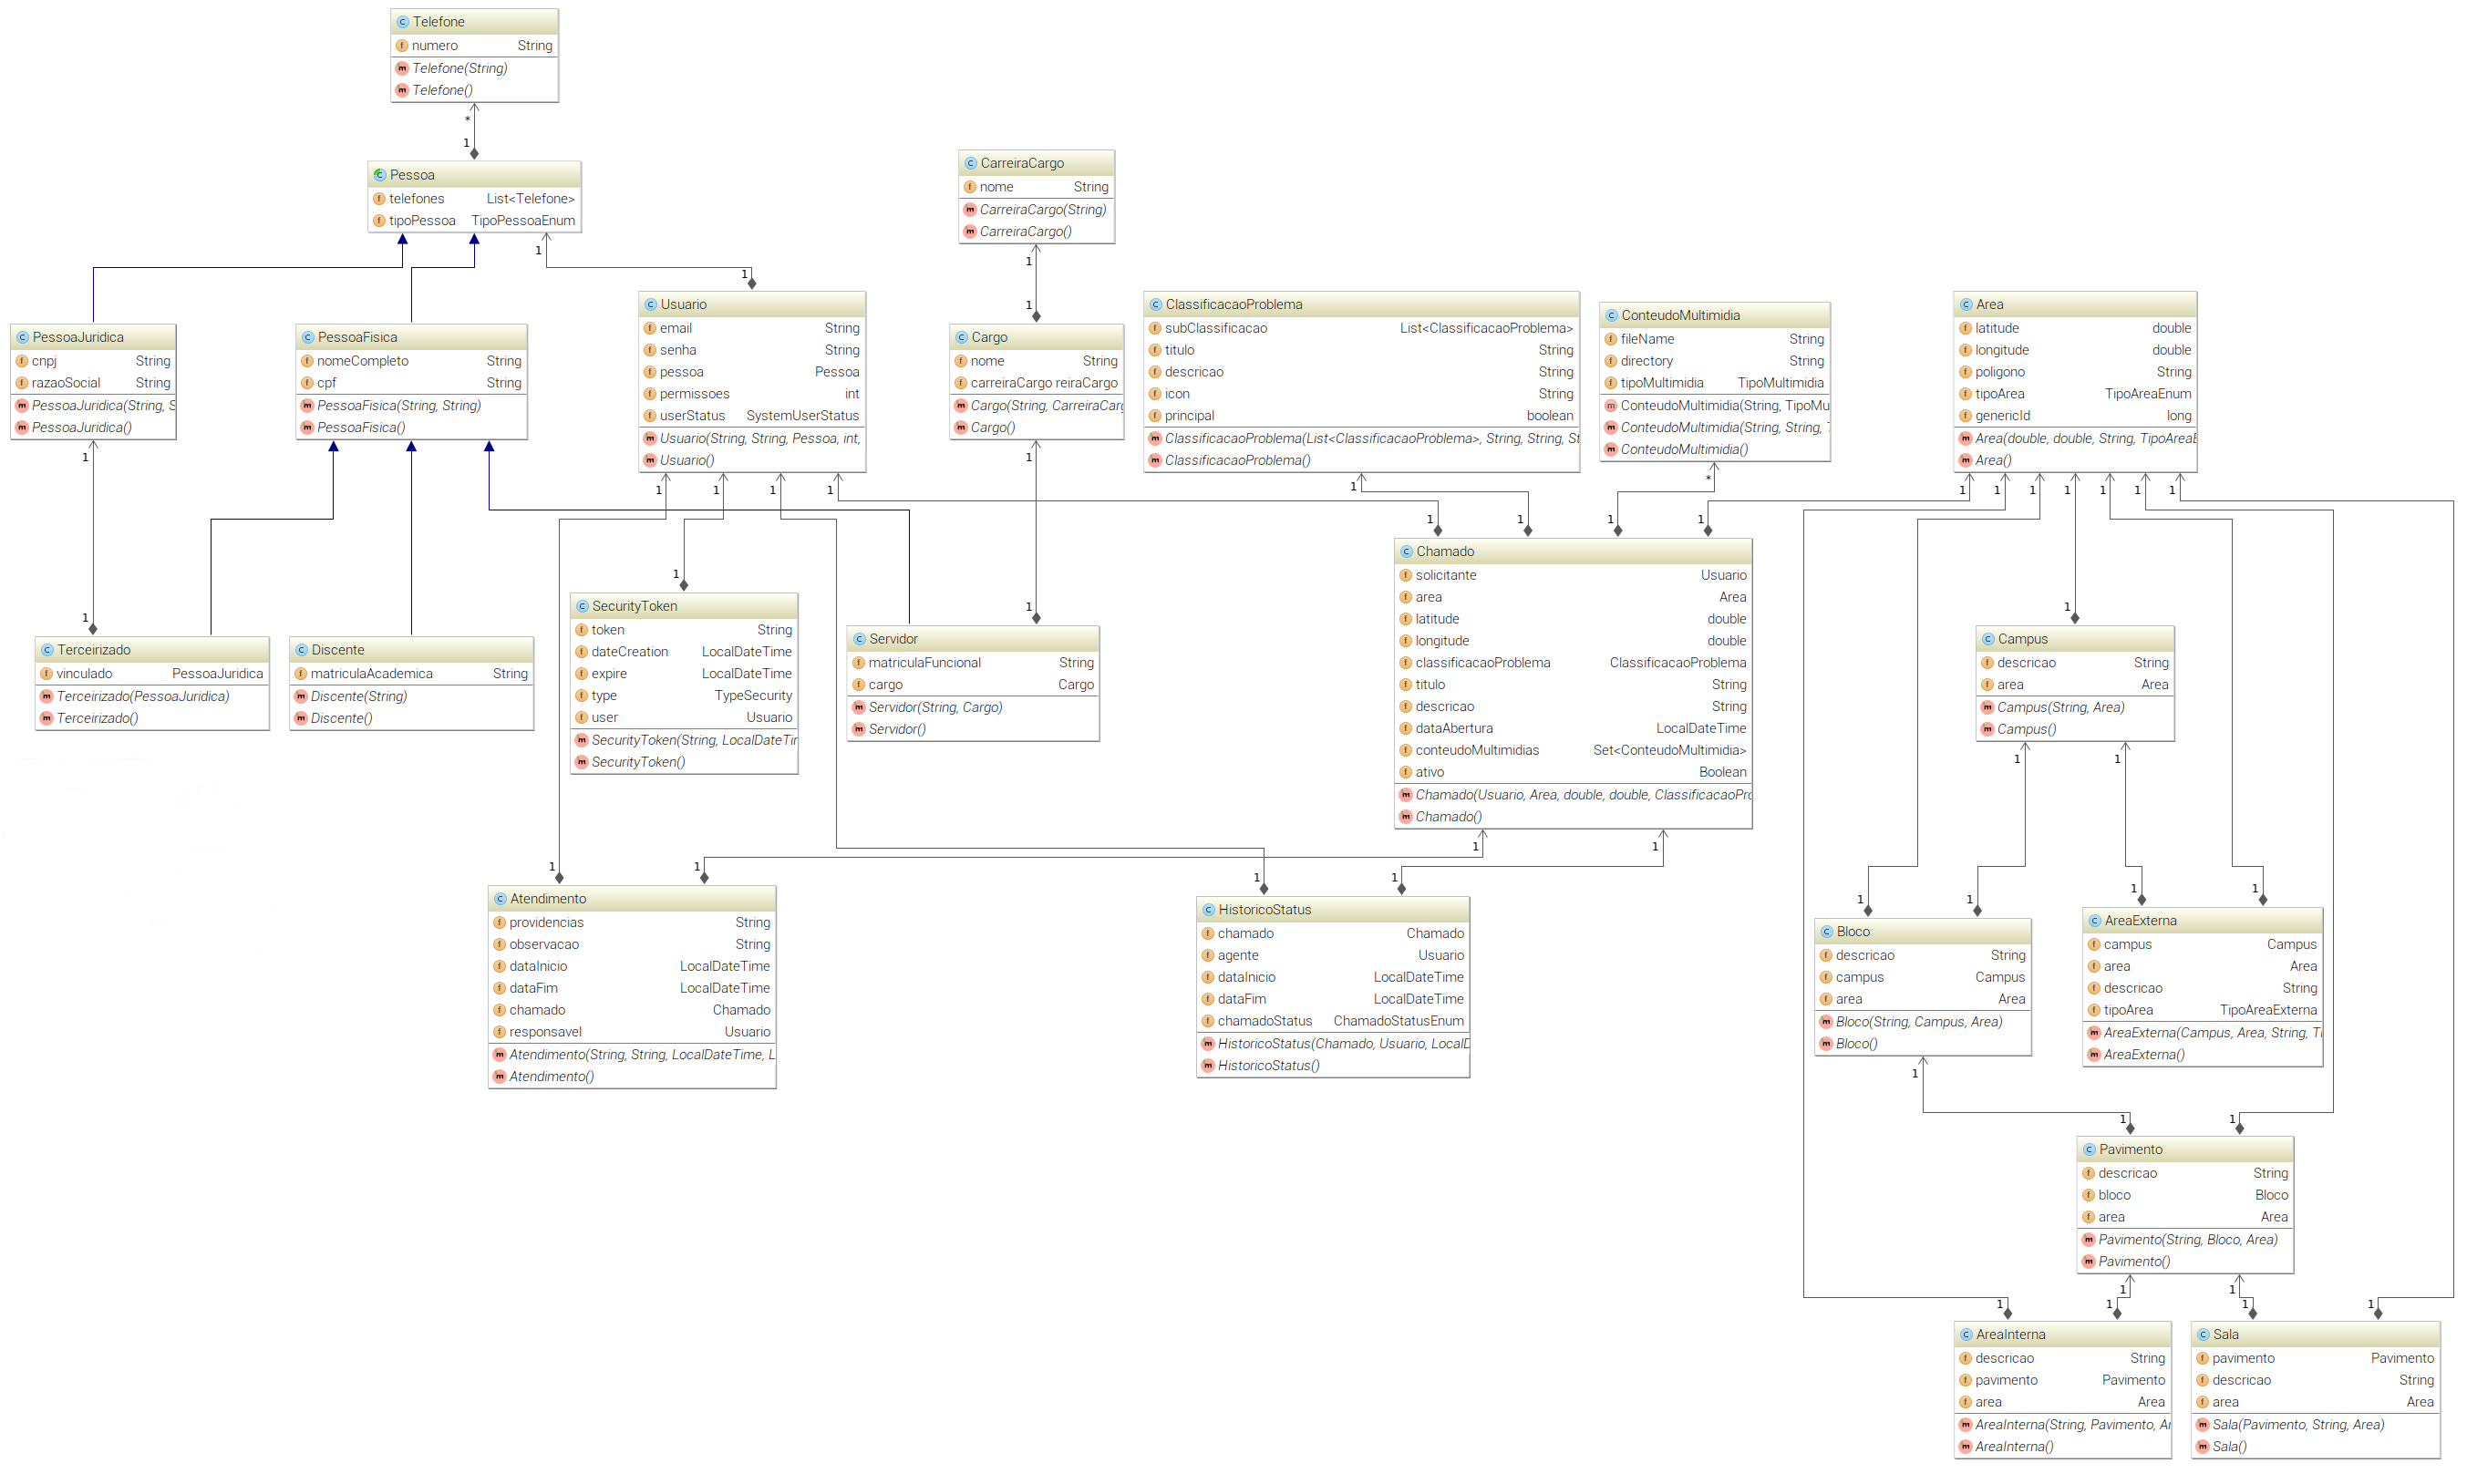
\includegraphics[angle=270, width=0.9\textwidth]{figuras/uft-servicos-diagram} 
 \caption{Diagrama de classes do sistema ``\acrshort{uft} Serviços'' web administrativo.}
 \label{diagram-web} 
\end{figure}

\subsection*{Diagrama de Atividade}

\noindent Para um melhor entendimento sobre o processo de criação de usuário e abertura de chamado realizado pelo ``\acrshort{uft} Serviços'', foi criado dois digramas de atividade que demonstram as atividades que podem ser realizados pelo usuário durante a utilização do sistema. Nos diagramas a seguir é exposto todo o procedimento realizado para o cadastro do usuário no sistema e o procedimento realizado para a abertura de um chamado. A seguir na Figura \ref{diagram-atividade} é apresentado os diagramas de atividades mencionados.

O primeiro diagrama de atividade apresentado na Figura \ref{diagram-atividade} exemplifica o processo de abertura de um chamado pelos usuários do sistema através do aplicativo móvel. O processo consiste na seleção de uma categoria de chamado e a validação do formulário através do preenchimento de informações como o título, descrição, localização e foto do chamado. Sendo que após a validação do formulário de abertura do chamado as informações são enviadas para o servidor de aplicação do sistema ``\acrshort{uft} Serviços''.

O diagrama apresentado na Figura \ref{diagram-web} apresenta o processo de cadastro e autenticação do usuário no aplicativo móvel, onde o processo consiste no preenchimento e validação do formulário de cadastro de usuário. Após a validação do formulário é enviado as informações para o servidor de aplicação e criado um novo usuário com o \textit{status} inativo. O sistema então envia um \textit{e-mail} de ativação do usuário, onde caso o usuário clique no \textit{link} de ativação o seu \textit{status} será mudado para ativo e consequentemente o usuário poderá realizar a autenticação no sistema.

\begin{figure}[H]
 \centering
 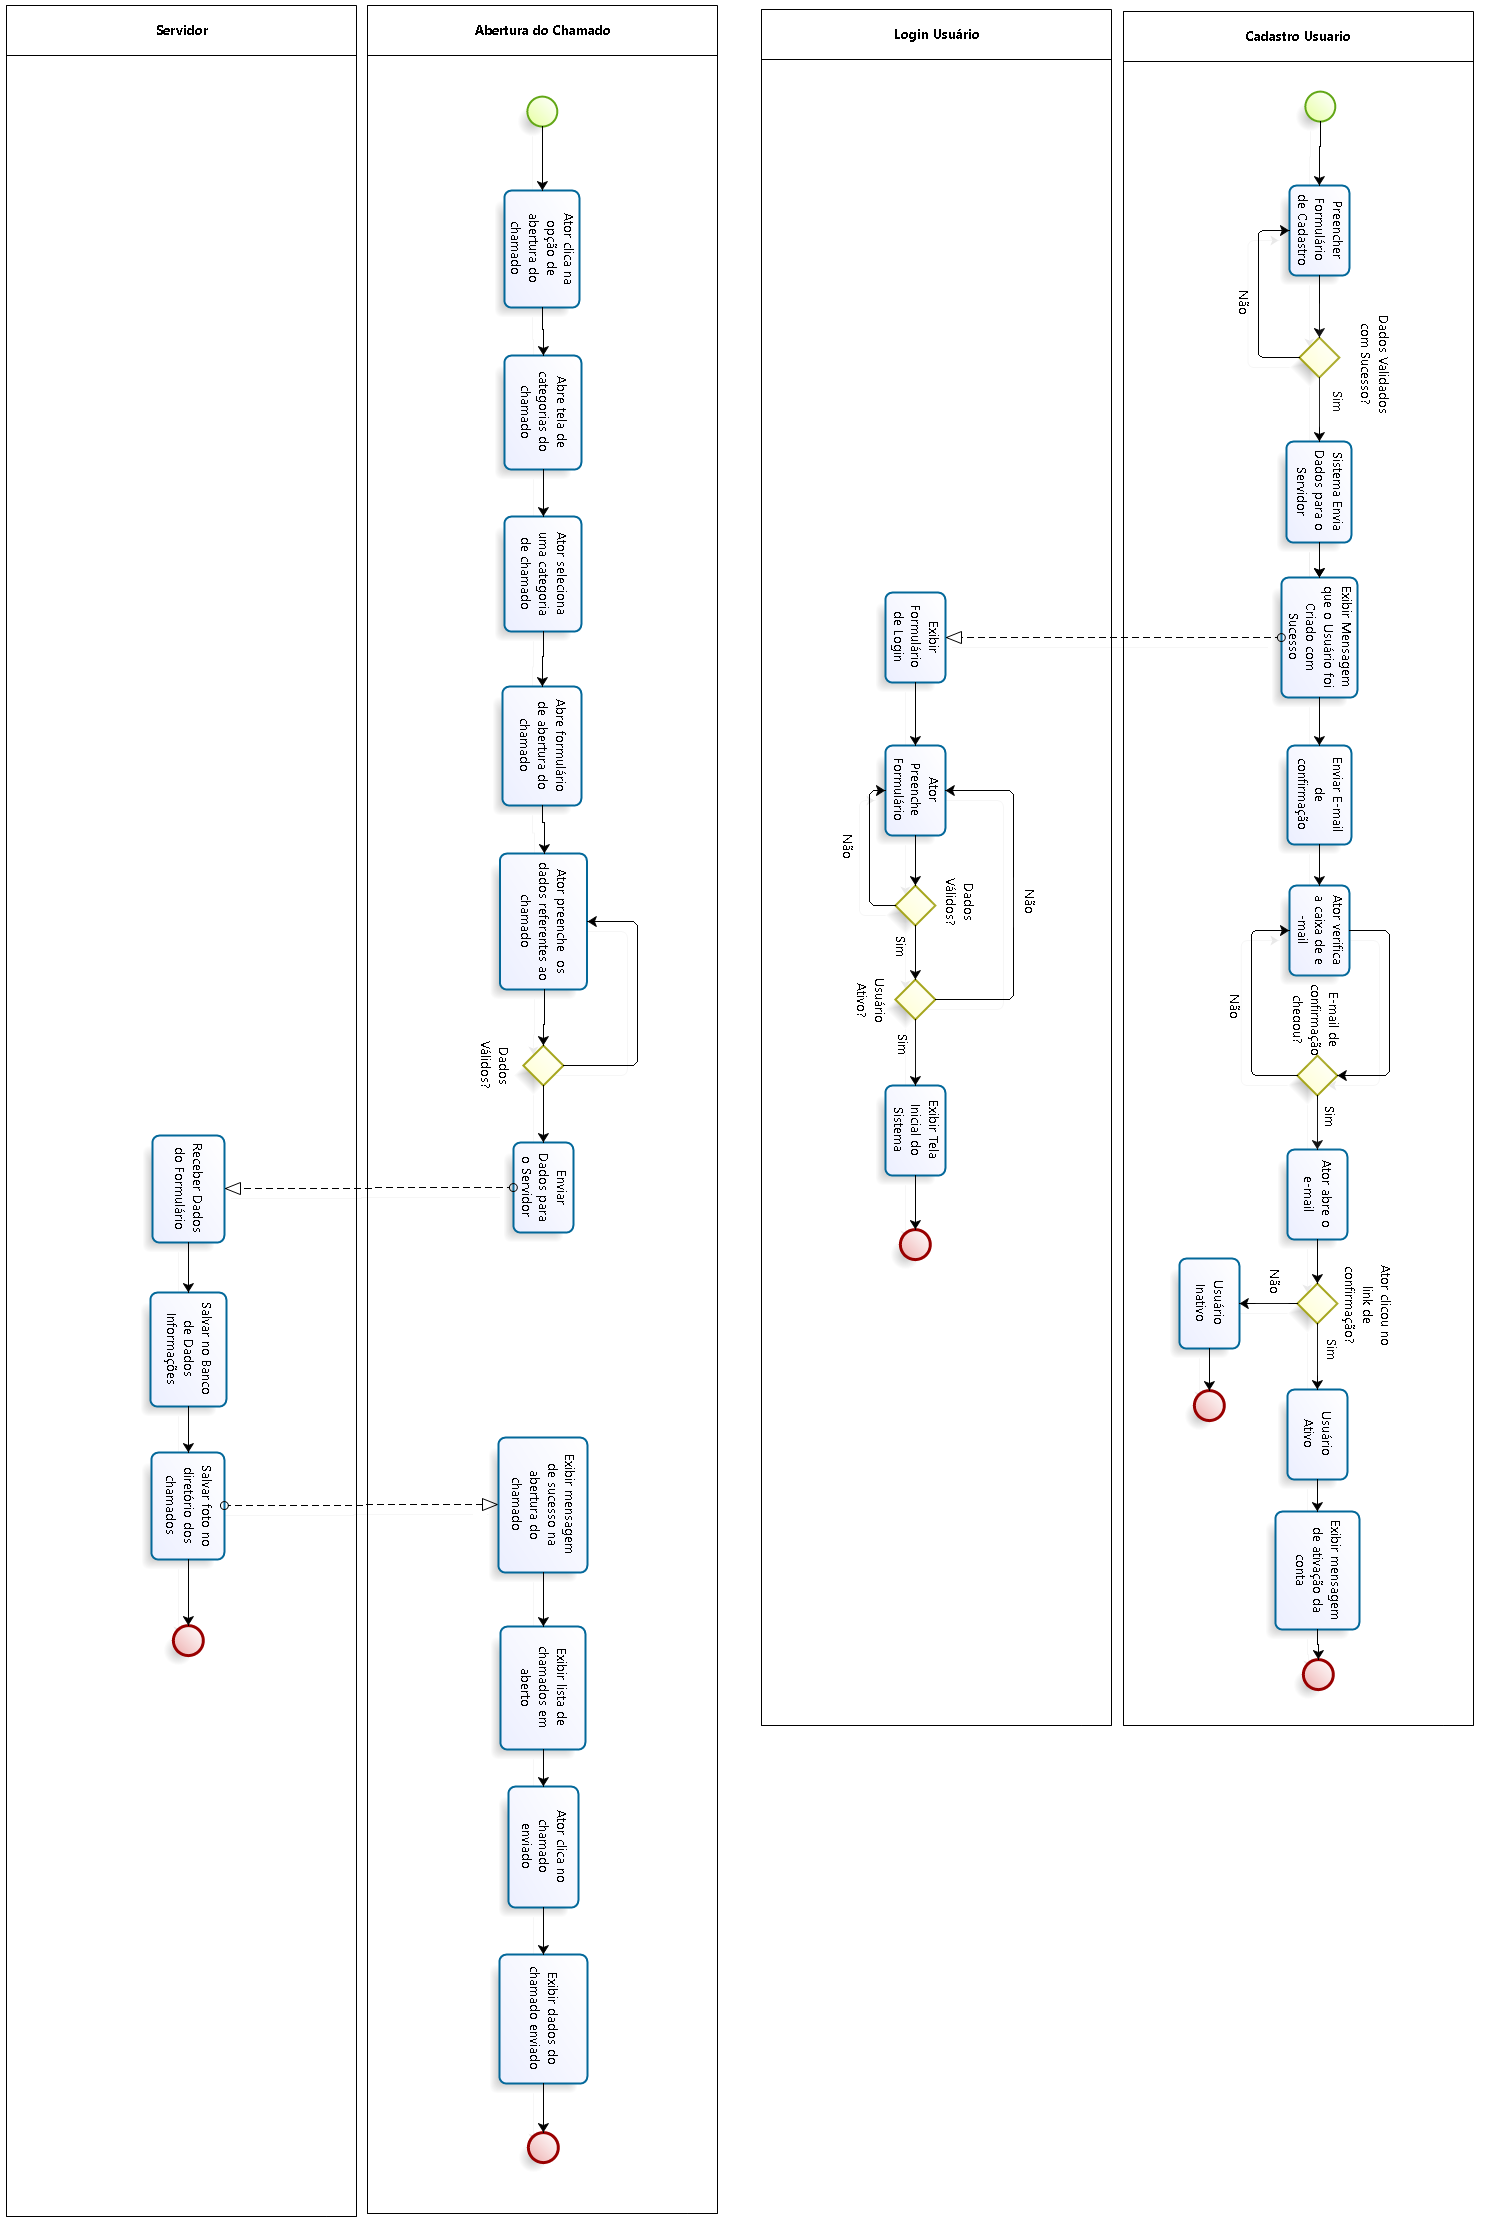
\includegraphics[width=1\textwidth]{figuras/atividade} 
 \caption{Diagramas de Atividade criação de usuário e autenticação e Processo de Abertura de Chamado.}
 \label{diagram-atividade} 
\end{figure}

\subsection*{Diagramas de Implantação}

\noindent O Diagramas de Implantação apresenta informações através da definição de nós, onde cada nó representa um módulo do sistema desenvolvido além de demonstrar os padrões e protocolos de comunicação em que cada nó faz com os demais. Como pode ser observado na Figura \ref{deployment_diagram} é apresentado modelo de diagrama de implantação adotado para a concepção do sistema ``\acrshort{uft} Serviços''.

\begin{figure}[H]
 \centering
 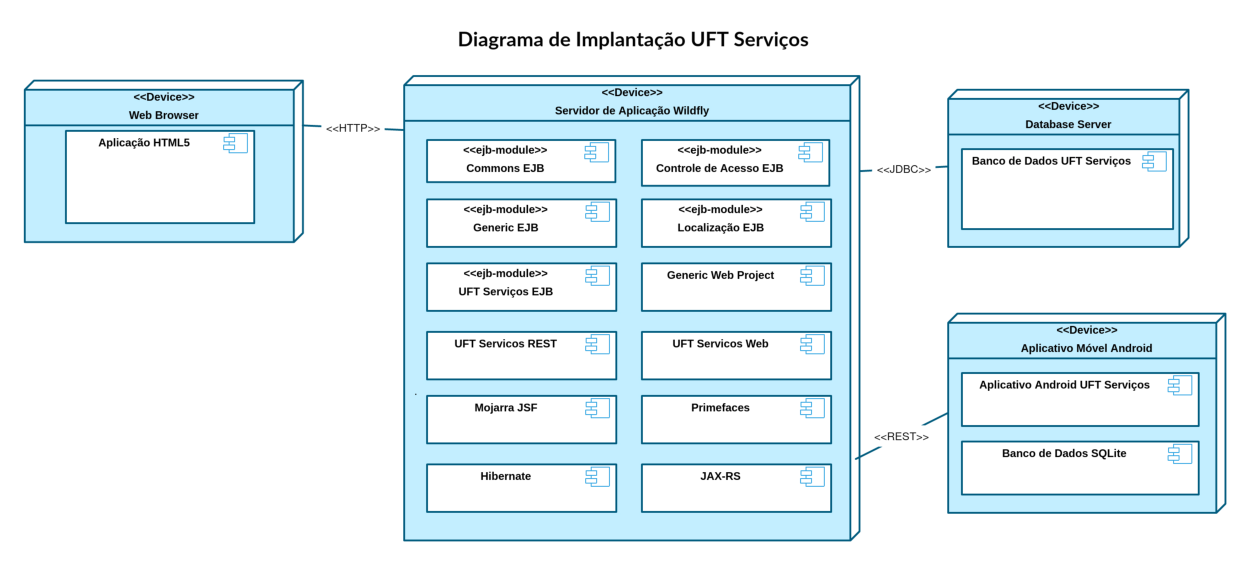
\includegraphics[width=1\textwidth]{figuras/deployment_diagram} 
 \caption{Diagramas de Implantação sistema ``\acrshort{uft} Serviços''.}
 \label{deployment_diagram} 
\end{figure}

Uma característica do sistema desenvolvido é o fato que a aplicação foi organizada em módulos \gls{ejb}, onde cada módulo \acrshort{ios} apresentado é responsável por uma tarefa específica no sistema. Outro ponto importante é os protocolos e padrões de comunicação adotado para comunicação do sistema, dentre eles está o protocolo \acrshort{http} e padrões de comunicação \acrshort{rest} e \gls{jdbc}.

\section{Ferramentas e Materiais}

\noindent Nesta seção é descrita as ferramentas utilizadas para o desenvolvimento do sistema ``\acrshort{uft} Serviços'', onde é descrito a funcionalidade de cada uma das ferramentas, as versões utilizadas no sistema e o motivo de sua utilização. Abaixo é listado todas as principais ferramentas que compõem o sistema ``\acrshort{uft} Serviços''.

\begin{enumerate}

    \item O \gls{javaee}\footnote{JavaEE: http://www.oracle.com/technetwork/java/javaee/overview/index.html} é um padrão de desenvolvimento de software corporativo oferecido pela Oracle para a comunidade de programadores Java. O Java EE é desenvolvido usando a \textit{Java Community Process} (JCP), através de contribuições de especialistas da indústria, organizações comerciais e comunidade de desenvolvedores de código \textit{open-source}.
    
    \item O \gls{jsf}\footnote{\acrshort{jsf}: https://javaserverfaces.java.net/} é um conjunto de especificações baseado no padrão MVC para construção de aplicações e interfaces \textit{web} com o usuário do lado cliente-servidor. O \acrshort{jsf} é baseado na abordagem de desenvolvimento orientado a componentes (\textit{component-based}) para construção de interfaces gráficas para a \textit{web}. O desenvolvimento de aplicações \acrshort{jsf} tem como base a orientação a eventos, característica essa que tem como propósito tornar mais prático o desenvolvimento de aplicações \textit{web} com o foco em oferecer aos desenvolvedores um ambiente de programação focado no desenvolvimento das regras de negócio da aplicação. A implementação padrão \acrshort{jsf} utilizada é o Mojarra 2.2.
    
    \item O Primefaces\footnote{Primefaces: http://www.primefaces.org/} é uma biblioteca \textit{open-source} de componentes que tem como propósito fornecer uma extensão aos componentes padrões presentes no \textit{Java Server Faces}.  Sua escolha foi feita devido a sua facilidade de utilização além da vasta opção de componentes presentes na biblioteca. A versão utilizada neste trabalho é a \textit{Primefaces Community} 5.3.
    
    \item O Materialize\footnote{Materialize: http://materializecss.com/} é uma biblioteca  \acrshort{css} para a criação de interfaces gráficas para \textit{web} utilizando o padrão de design Material Design\footnote{Material Desing: https://material.google.com/}. O motivo da escolha do Materialize foi por conta da facilidade de criação de layouts em HTML5 baseado no padrão Material Design.
    
    \item O Simple Grid é uma ferramenta em  \acrshort{css} para criação de \textit{grids} para organização de \textit{layout} da aplicação \textit{web} do ``\acrshort{uft} Serviços''. Sua escolha foi feita devido sua simplicidade para a criação de \textit{grid} e também por seu tamanho ser pequeno em relação a outras bibliotecas  \acrshort{css} com a mesma finalidade.
    
    \item O \gls{jpa}\footnote{JPA: http://www.oracle.com/technetwork/java/javaee/tech/persistence-jsp-140049.html} é uma especificação que fornece aos desenvolvedores um ambiente de desenvolvimento \gls{poo} baseado no \gls{pojo}. O modelo \acrshort{pojo} tem como objetivo tornar simplificado a forma como os desenvolvedores lidam com a persistência de dados através de abstrações do modelo banco de dados relacional para o ambiente de desenvolvimento orientado a objeto. A versão do \acrshort{jpa} utilizada no projeto é a implementação desenvolvida pela Red Hat\footnote{Red Hat: https://www.redhat.com/}, o Hibernate\footnote{Hibernate: http://hibernate.org/} 5.
    
    \item O sistema de banco de dados relacional utilizado neste trabalho é o o PostgreSQL\footnote{PostgreSQL: http://www.postgresql.org/}. Sua escolha foi feita devido sua estabilidade e sua capacidade de manter a integridade dos dados. Outra motivação para escolha do PostgreSQL é sua ampla documentação e comunidade de usuários ativa, além do fato dele ser o banco de dados \textit{open-source} mais utilizado no mundo. A versão do PostgreSQL utilizada neste projeto é a 9.5.
    
    \item O Apache Maven\footnote{Apache Maven: https://maven.apache.org/} é uma ferramenta para gerenciamento de dependências Java de uso fundamental para construções do sistema \textit{web} do ``\acrshort{uft} Serviços''. Suas funcionalidades vão além de um gerenciamento de dependências, mas também como uma ferramenta para automatização de compilação (build) de projetos construídos em Java. A versão do Apache Maven utilizado no projeto é a 3.3.9.
    
    \item O Apache Shiro\footnote{Apache Shiro: http://shiro.apache.org/} é um \textit{framework} de controle de acesso utilizado no sistema \textit{web} do ``\acrshort{uft} Serviços''. A versão utilizada neste trabalho é a 1.2.4.
    
    \item O Pretty Faces\footnote{Pretty Faces: http://www.ocpsoft.org/prettyfaces/} é uma ferramenta para criação de URL's amigáveis através da definição de contextos específicos para cada uma das páginas do sistema. A versão utilizada neste trabalho é a 2.0.12.
    
    \item O JAX-RS\footnote{JAX-RS: https://jax-rs-spec.java.net/} é uma API e especificação para construção de serviços \textit{web} de comunicação REST-API para a plataforma Java. A versão utilizada neste trabalho é a 2.0.
    
    \item O servidor \textit{web container} utilizado neste trabalho é o Wildfly\footnote{Wildfly: http://wildfly.org/}. Sua utilização se dá pelo fato de sua ampla comunidade de usuários e números de \textit{releases} e correções feitas periodicamente. A versão do Wildfly utilizado neste trabalho é a 10.
    
    \item O servidor para integração contínua utilizado para realização dos \textit{builds} e testes automatizados do sistema ``\acrshort{uft} Serviços'' é o Jenkins\footnote{Jenkins: https://jenkins.io/}, sua utilização foi feita devido ser o sistema de integração contínua de \textit{software} de código aberto mais popular no mercado, além de suas diversas possibilidades de configuração e sistema de \textit{plugins}. A versão do Jenkins utilizada neste projeto é a 2.0.
    
    \item O Android \acrshort{sdk}\footnote{Android \acrshort{sdk}: http://developer.android.com/intl/pt-br/sdk/index.html} é a biblioteca padrão utilizada para desenvolvimento de aplicativos para a plataforma Android OS.
    
    \item A IDE utilizada para desenvolvimento da aplicação móvel é o Android Studio\footnote{Android Studio: http://developer.android.com/intl/pt-br/sdk/index.html}. Sua utilização se dá pelo fato de seu amplo suporte e por ser a \acrshort{ide} oficial para desenvolvimento de aplicativos móveis para plataforma Android. A versão utilizada para desenvolvimento do aplicativo móvel ``\acrshort{uft} Serviços'' é a 2.1.
    
    \item A \acrshort{ide} utilizada para desenvolvimento do sistema \textit{web} e REST do ``\acrshort{uft} Serviços'' é o Netbeans\footnote{Netbeans: https://netbeans.org/}. Sua escolha foi feita devido seu amplo suporte à criação de aplicações Java e sua estabilidade e funcionalidades oferecidas pela \acrshort{ide}. A versão do Netbeans utilizada neste trabalho é a 8.1.
    
    \item O Ubuntu OS\footnote{Ubuntu: http://www.ubuntu.com/} é um sistema operacional \textit{open-source} baseado no \textit{kernel} Linux mais utilizado no mundo. Sua utilização é feita tanto no ambiente de desenvolvimento como no ambiente de produção, a versão utilizada no projeto é o Ubuntu 14.04.4 LTS.
    
    \item O Netdata\footnote{Netadata: https://github.com/firehol/netdata} é um sistema de monitoramento \textit{open-source} de \textit{hardware} e rede. Sua escolha foi feita devido sua facilidade de configuração e o número de gráficos que é apresentado pelo sistema.
    
    \item O Google \textit{Analytics}\footnote{Google Analytics: https://analytics.google.com/} é um sistema \textit{web} para monitoramento de acesso dos usuários do aplicativo móvel do ``\acrshort{uft} Serviços''. Sua utilização foi feita devido a facilidade de configuração da API de monitoramento no aplicativo Android e por fornecer diversas informações sobre o usuário como sexo, idade e região. Outra motivação para escolha da ferramenta é por conta do Google \textit{Analytics} oferecer em detalhes informações como o rastreamento de exceções, quais telas o usuário acessou durante o uso do aplicativo e a quantidade usuários que estão utilizando o sistema no momento.

\end{enumerate}

\section*{Considerações finais sobre o capítulo}

\noindent Neste capítulo foi apresentado os principais conceitos utilizados para a construção do sistema ``\acrshort{uft} Serviços'', sendo apresentado o ambiente computacional, os métodos, os diagramas \acrshort{uml} e as ferramentas utilizadas no sistema.

A utilização do \acrshort{itil} v3, \textit{Scrum} e aplicação do teste de usabilidade  \acrshort{sus} foram de grande importância para o desenvolvimento e implantação do \textit{software}. Através da aplicação dos conceitos apresentados foi possível obter uma base sólida quando a organização dos processos e serviços utilizados para implantação e manutenção do ``\acrshort{uft} Serviços''.